\section{Исследование парметров барьеров}

\subsection{Исследование ширины барьеров}
Ширина барьеров уменьшает вероятность прохождения электрона сквозь барьер и величину тока соответсвенно. Рассмотрим РТГС с шириной барьеров:
\begin{enumerate}
	\item 10 монослоев;
	\item 7 монослоев;
	\item 5 монослоев;
	\item 3 монослоев.
\end{enumerate}

\subsubsection{Прозрачность РТГС}
\begin{figure}[h]
	\centering
	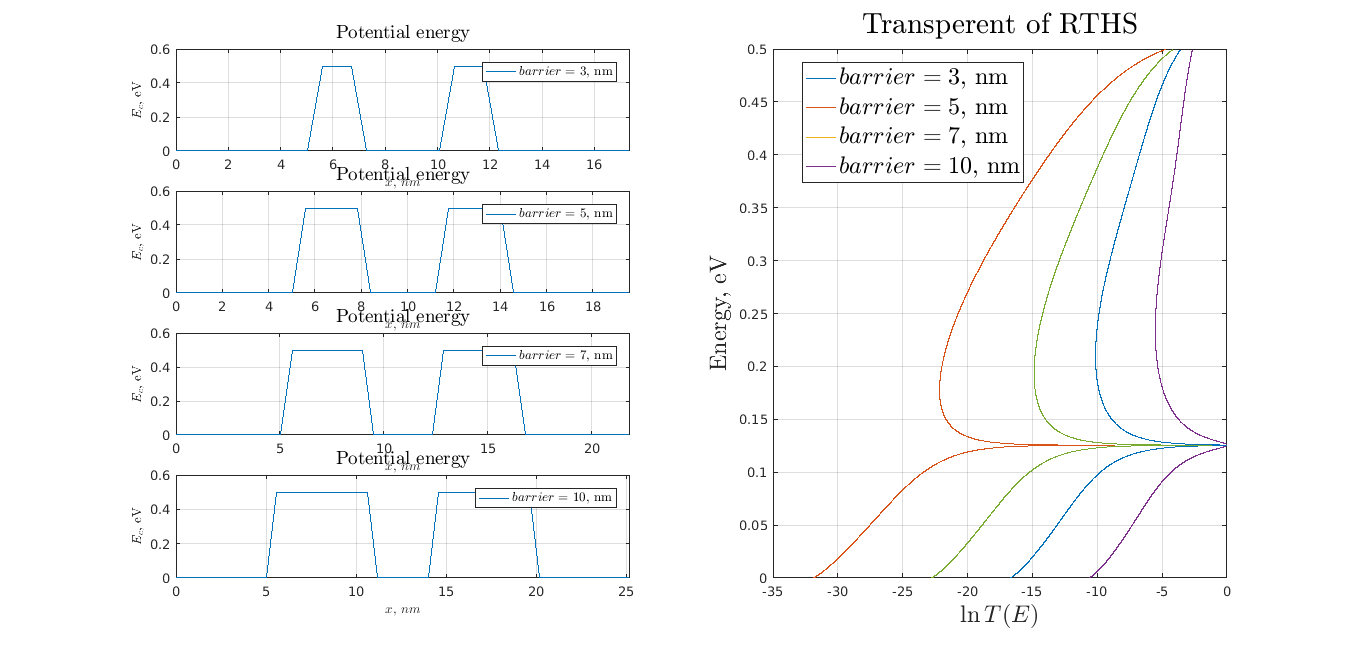
\includegraphics[scale=0.5]{qbwt.png}
	\caption{Прозрачность РТГС при различных ширинах потенциальных барьеров}
	\label{fig:qbwt}
\end{figure}

\subsubsection{ВАХ РТГС}
\begin{figure}[h]
	\centering
	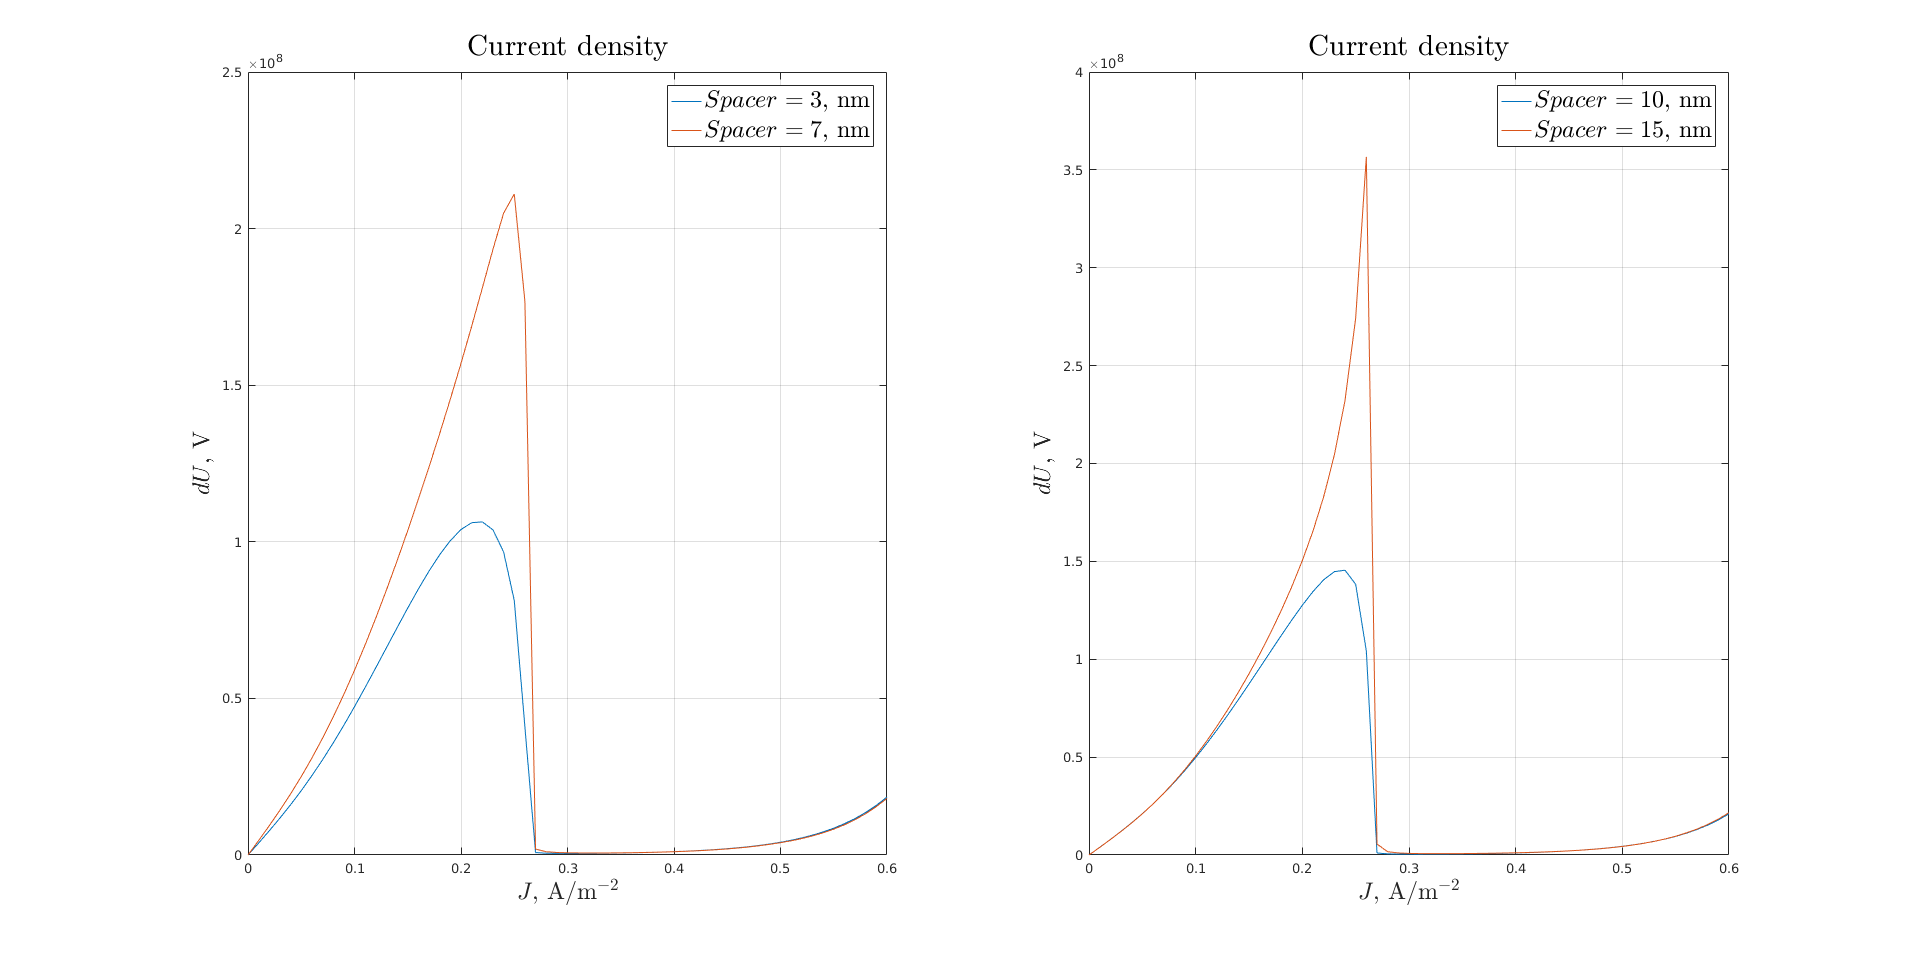
\includegraphics[scale=0.5]{qbwj.png}
	\caption{Плотность тока через РТГС при различных ширинах потенциальных барьеров}
	\label{fig:qbwj}
\end{figure}